\section{TXLWizard Example}
The following code demonstrates a simple example usage of the ``TXLWizard'' for
generating TXL files with python code. \\
The code can be found in the file \myPath{Content/Example\_Simple.py}.\\
The resulting image is shown in Figure \ref{fig:TXLWizardSimpleExample}.
A more advanced example is shown in Section \ref{sec:AppendixTXLWizardExampleAdvanced}
\lstinputlisting[language=Python]{Content/Example_Simple.py}


\begin{figure}[!htbp]
    \centering
     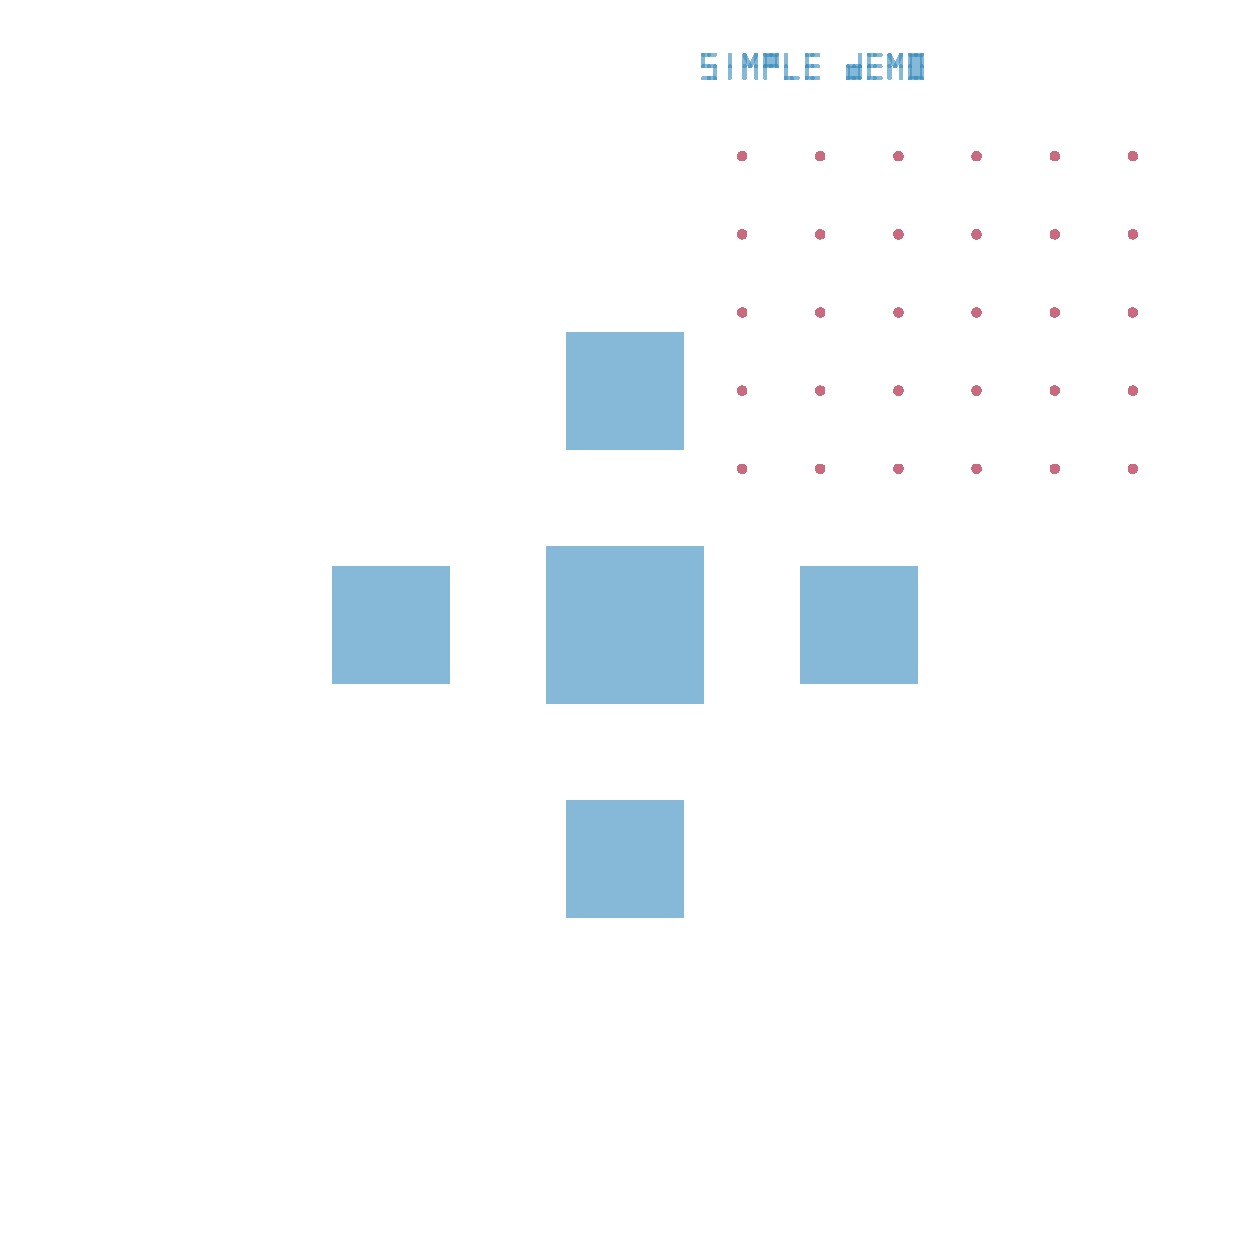
\includegraphics[width=\textwidth]{Content/Masks/Example_Simple.pdf}
    \caption{Simple Example: Generated Mask}
    \label{fig:TXLWizardSimpleExample}
\end{figure}